\documentclass[12pt]{book}

\newcommand{\thetitle}{Think Java: How to Think Like a Computer Scientist}
\title{\thetitle}

\newcommand{\theauthors}{Allen Downey and Chris Mayfield}
\author{\theauthors}

\newcommand{\theversion}{Version 6.0 Draft -- \today}
\date{\theversion}

\usepackage{geometry}
\geometry{
    width=5.5in,
    height=8.5in,
    hmarginratio=3:2,
    vmarginratio=1:1,
    includehead=true,
    headheight=15pt
}

% paragraph spacing
\setlength{\parindent}{0pt}                      % 17.62482pt
\setlength{\parskip}{12pt plus 4pt minus 4pt}    % 0.0pt plus 1.0pt
\linespread{1.05}
\def\arraystretch{1.5}

% list spacing
\setlength{\topsep}{5pt plus 2pt minus 3pt}      % 10.0pt plus 4.0pt minus 6.0pt
\setlength{\partopsep}{-6pt plus 2pt minus 2pt}  %  3.0pt plus 2.0pt minus 2.0pt
\setlength{\itemsep}{0pt}                        %  5.0pt plus 2.5pt minus 1.0pt

% these are copied from tex/latex/base/book.cls
% all I changed is afterskip
\makeatletter
\renewcommand{\section}{\@startsection {section}{1}{\z@}%
    {-3.5ex \@plus -1ex \@minus -.2ex}%
    {0.7ex \@plus.2ex}%
    {\normalfont\Large\bfseries}}
\renewcommand\subsection{\@startsection{subsection}{2}{\z@}%
    {-3.25ex\@plus -1ex \@minus -.2ex}%
    {0.3ex \@plus .2ex}%
    {\normalfont\large\bfseries}}
\renewcommand\subsubsection{\@startsection{subsubsection}{3}{\z@}%
    {-3.25ex\@plus -1ex \@minus -.2ex}%
    {0.3ex \@plus .2ex}%
    {\normalfont\normalsize\bfseries}}
\makeatother

% table of contents vertical spacing
\usepackage{tocloft}
\setlength\cftparskip{8pt plus 4pt minus 4pt}

% The following line adds a little extra space to the column
% in which the Section numbers appear in the table of contents
\makeatletter
\renewcommand{\l@section}{\@dottedtocline{1}{1.5em}{3.0em}}
\makeatother

% customize page headers
\usepackage{fancyhdr}
\pagestyle{fancyplain}
\renewcommand{\chaptermark}[1]{\markboth{Chapter \thechapter ~~ #1}{}}
\renewcommand{\sectionmark}[1]{\markright{\thesection ~~ #1}}
\lhead[\fancyplain{}{\bfseries\thepage}]%
      {\fancyplain{}{\bfseries\rightmark}}
\rhead[\fancyplain{}{\bfseries\leftmark}]%
      {\fancyplain{}{\bfseries\thepage}}
\cfoot{}
%\rfoot{\textcolor{gray}{\tiny ThinkJava Draft \today}}

% balanced index with TOC entry
\usepackage{makeidx}
\makeindex
%\usepackage[totoc]{idxlayout}

% automatically index glossary terms
\newcommand{\term}[1]{%
\index{#1}
\item[#1:]}
% TODO: doesn't work with plastex
%\newcommand{\term}[1]{\item[#1:]}

% where to find graphics
\usepackage{graphicx}
%\graphicspath{{figs/}}

%% tweak spacing of figures and captions
%\usepackage{floatrow}
%\usepackage{caption}
%\captionsetup{
%    font=small,
%    labelformat=empty,
%    justification=centering,
%    skip=4pt
%}

% format end of chapter excercises
\usepackage{amsmath}
\usepackage{amsthm}
\newtheoremstyle{exercise}
  {12pt}        % space above
  {12pt}        % space below
  {}            % body font
  {}            % indent amount
  {\bfseries}   % head font
  {}            % punctuation
  {12pt}        % head space
  {}            % custom head
\theoremstyle{exercise}
\newtheorem{exercise}{Exercise}[chapter]

% colors for code listings and output
\usepackage{xcolor}
\definecolor{bgcolor}{HTML}{FAFAFA}
\definecolor{comment}{HTML}{007C00}
\definecolor{keyword}{HTML}{0000FF}
\definecolor{strings}{HTML}{B20000}

% syntax highlighting in code listings
\usepackage{textcomp}
\usepackage{listings}
\lstset{
    language=java,
    basicstyle=\ttfamily,
    backgroundcolor=\color{bgcolor},
    commentstyle=\color{comment},
    keywordstyle=\color{keyword},
    stringstyle=\color{strings},
    columns=fullflexible,
    keepspaces=true,
    showstringspaces=false,
    upquote=true,
    aboveskip=\parskip,
    belowskip=\parskip
}

% code listing environments
\lstnewenvironment{code}
{\minipage{\linewidth}}
{\endminipage}
\lstnewenvironment{stdout}
{\lstset{commentstyle=,keywordstyle=,stringstyle=}\minipage{\linewidth}}
{\endminipage}

% pdf hyperlinks, table of contents, and document properties
\usepackage[pdftex]{hyperref}
\hypersetup{%
  pdftitle={\thetitle},
  pdfauthor={\theauthors},
  pdfsubject={\theversion},
  pdfkeywords={},
  bookmarksopen=false,
  colorlinks=true,
  citecolor=black,
  filecolor=black,
  linkcolor=black,
  urlcolor=blue
}

% inline syntax formatting
\newcommand{\java}[1]{\lstinline{#1}} %\end{
%\newcommand{\java}[1]{\verb"#1"}
%\newcommand{\java}[1]{{\tt #1}}

\begin{document}
\setcounter{chapter}{12}


\chapter{Objects of Arrays}

\index{array!of Cards}

Previously we looked at algorithms for searching for a particular \java{Card} in an array of \java{Card} objects.
It turns out that an array of \java{Card}s is not only useful for representing an entire deck, but also for representing a subdeck (i.e., part of the deck).
For example, we can use a separate array for each player to remember which \java{Card}s they have been dealt.

In this chapter, we will take another step toward object-oriented programming.
We will also develop algorithms for shuffling and sorting decks of cards.
While reading the following sections, we recommend that you create a {\tt Deck.java} file and paste in all the examples.
You will need {\tt Card.java} from the previous chapter for it to compile.

%So many of the examples are non-idiomatic; that is, they are not good Java.
%This transitional form should help you learn, but don't write code like this.

%You can download the code in this chapter from \url{http://thinkapjava.com/code/Card2.java}.


\section{The Deck class}
\label{deck}

The main idea of this chapter is to create a \java{Deck} class that contains (encapsulates) an array of \java{Card}s.
The initial class definition looks like this:

\begin{code}
public class Deck {
    private Card[] cards;

    public Deck(int n) {
        this.cards = new Card[n];
    }
}
\end{code}

\index{constructor}
\index{state diagram}

The constructor initializes the instance variable with an array of cards, but it doesn't create any cards.
Here is a state diagram showing what a \java{Deck} looks like with no cards:

\begin{center}
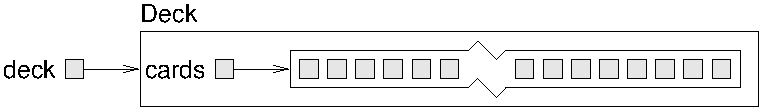
\includegraphics{figs/deckobject.pdf}
\end{center}

We will also provide a default constructor that makes a standard 52-card deck and populates it with \java{Card} objects:

\begin{code}
    public Deck() {
        this.cards = new Card[52];
        int index = 0;
        for (int suit = 0; suit <= 3; suit++) {
            for (int rank = 1; rank <= 13; rank++) {
                cards[index] = new Card(suit, rank);
                index++;
            }
        }
    }
\end{code}

\index{new}
\index{statement!new}

This method is similar to \java{makeDeck} from the previous chapter; we just changed the syntax to make it a constructor.
To invoke it, we apply the \java{new} operator:

\begin{code}
    Deck deck = new Deck();
\end{code}

\index{printDeck}

Now it makes sense to put the methods that pertain to \java{Deck}s in the \java{Deck} class definition.
Looking at the methods we have written so far, one obvious candidate is \java{printDeck} (Section~\ref{printdeck}).
Here's how it looks, rewritten to work with a \java{Deck}:

\begin{code}
    public static void printDeck(Deck deck) {
        for (int i = 0; i < deck.cards.length; i++) {
            Card.printCard(deck.cards[i]);
        }
    }
\end{code}

The main change is the type of the parameter: from \java{Card[]} to \java{Deck}.
As a result, we can no longer use \java{deck.length} to get the length of the array.
The Deck object contains an array, but it is not an array by itself.
So we have to write \java{deck.cards.length} to extract the array from the \java{Deck} object and get the length of the array.
For the same reason, we have to use \java{deck.cards[i]} to access an element of the array, rather than just \java{deck[i]}.
%The last change is that the invocation of \java{printCard} has to say explicitly that \java{printCard} is defined in the \java{Card} class.


\section{Subdecks of cards}
\index{subdeck}

How should we represent a subset of a full deck?
One possibility is to create a new class, but it would be very similar to \java{Deck}.
A better option is to reuse the \java{Deck} class, but have fewer than 52 cards.

We might want a method, \java{subdeck}, that takes a Deck and a range of indexes.
It will return a new Deck with the specified subset of the cards:

\begin{code}
public static Deck subdeck(Deck deck, int low, int high) {
    Deck sub = new Deck(high - low + 1);

    for (int i = 0; i < sub.cards.length; i++) {
        sub.cards[i] = deck.cards[low + i];
    }
    return sub;
}
\end{code}

Note that the length of the subdeck is \java{high - low + 1}, because both the low card and the high card are included.
This sort of computation can be confusing, and forgetting the \java{+ 1} often leads to ``off-by-one'' errors.
Drawing a picture is usually the best way to avoid them.

\index{constructor}
\index{overloading}

Because the first line provides an argument with \java{new}, the non-default constructor gets invoked.
It simply allocates the array without allocating any cards.
Inside the \java{for} loop, the subdeck gets populated with copies of the references from the deck.

The following is a state diagram of a subdeck being created with the parameters \java{low = 3} and \java{high = 7}.
The result is a hand with 5 cards that are {\em shared} with the original deck, i.e., they are aliased.

\begin{center}
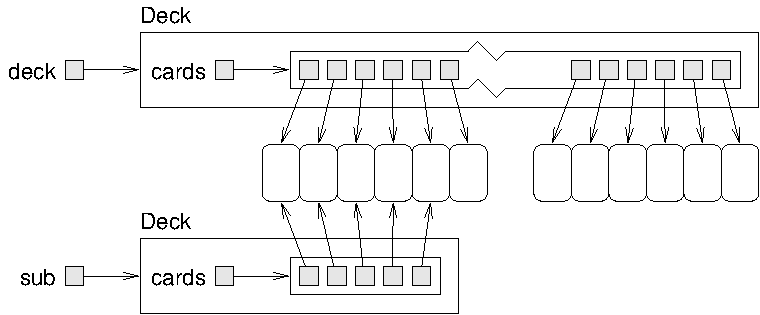
\includegraphics{figs/subdeck.pdf}
\end{center}

\index{aliasing}
\index{reference}

Aliasing is not always a good idea, because changes to shared objects are reflected in multiple decks.
However, since we designed \java{Card} objects to be immutable, they will never change.
So for \java{Card}s, \java{String}s, and other immutable objects, aliasing is an efficient choice.


\section{Shuffling and dealing}
\label{shuffle}

\index{shuffle}

For most card games you need to be able to shuffle the deck, i.e., put the cards in a random order.
In Section~\ref{random} we saw how to generate random numbers, but it is not obvious how to use them to shuffle a deck.

One possibility is to model the way humans shuffle, which is usually dividing the deck in two and then choosing alternately from each deck.
Since humans usually don't shuffle perfectly, after about seven iterations the order of the deck is pretty well randomized.

But a computer program would have the annoying property of doing a perfect shuffle every time, which is not really very random.
In fact, after eight perfect shuffles, you would find the deck back in the order you started in!
(For more information, see \url{http://en.wikipedia.org/wiki/Faro_shuffle}.)

\index{pseudocode}

A better shuffling algorithm is to traverse the deck one card at a time, and at each iteration choose two cards and swap them.
Here is an outline of how this algorithm works.
To sketch the program, we will use a combination of Java statements and English.
This technique is sometimes called {\bf pseudocode}.

\begin{code}
    for each card index {
        // choose a number between i and deck length - 1
        // swap the ith card and the randomly-chosen card
    }
\end{code}

\index{randomInt}
\index{swapCards}

The nice thing about pseudocode is that it often makes clear what methods you are going to need.
In this case, we need something like \java{randomInt}, which chooses a random integer between \java{low} and \java{high}, and \java{swapCards}, which takes two indexes and switches the cards at those positions.

\index{program development}

This process---writing pseudocode first and then writing methods to make it work---is called {\bf top-down development} (see \url{http://en.wikipedia.org/wiki/Top-down_and_bottom-up_design}).

\index{shuffling}
\index{dealing}

Assuming that we have a method called \java{shuffleDeck} that takes a deck as an argument and shuffles it, we can use it to deal two players:

\begin{code}
    Deck deck = new Deck();
    shuffleDeck(deck);

    Deck hand1 = subdeck(deck, 0, 4);
    Deck hand2 = subdeck(deck, 5, 9);
    Deck pack = subdeck(deck, 10, 51);
\end{code}

This code puts the first five cards in one hand, the next five cards in the other, and the rest into the pack.

When you thought about dealing, did you think we should give one card to each player in the round-robin style that is common in real card games?
The round-robin convention is intended to mitigate imperfect shuffling and make it more difficult for the dealer to cheat.

This example is a useful reminder of one of the dangers of engineering metaphors.
Sometimes we impose restrictions on computers that are unnecessary, or expect capabilities that are lacking, because we unthinkingly extend a metaphor past its breaking point.


\section{Selection sort algorithm}
\label{sorting}

\index{selection sort}
\index{sort!selection}

Now that we have messed up the deck, we need a way to put it back in order.
There is an algorithm for sorting that is ironically similar to the algorithm for shuffling.
It's called {\bf selection sort} because it works by traversing the array repeatedly and selecting the lowest (or highest) remaining card each time.

During the first iteration, we find the lowest card and swap it with the card in the 0th position.
During the \java{i}th, we find the lowest card to the right of $i$ and swap it with the $i$th card.
Here is pseudocode for selection sort:

\begin{code}
    for each card index {
        // find the lowest card at or to the right of i
        // swap the ith card and the lowest card found
    }
\end{code}

\index{helper method}
\index{method!helper}

Again, the pseudocode helps with the design of the {\bf helper methods}.
In this case we can use \java{swapCards} again, so we only need one new method that takes an array of cards and an index where it should start looking.
We'll call that method \java{indexLowestCard}.

Rather than show you the actual source code, we will leave the implementation as an exercise.


\section{Merging sorted decks}
\label{mergesort}

\index{efficiency}
\index{sorting}
\index{mergesort}

Selection sort is a simple algorithm that turns out not to be very efficient.
To sort $n$ items, it has to traverse the array $n$ times.
Each traversal takes an amount of time that is proportional to $n$.
The total time, therefore, is proportional to $n^2$.

In the next two sections, we'll consider a more efficient algorithm called {\bf mergesort}.
To sort $n$ items, mergesort takes time proportional to $n \log_2 n$.
That may not seem impressive, but as $n$ gets big, the difference between $n^2$ and $n \log_2 n$ can be enormous.
For example, $\log_2$ of one million is around 20.
So if you had to sort a million numbers, selection sort would require one trillion steps versus only 20 million for mergesort.

The basic idea behind mergesort is this: if you have two subdecks, each of which has already been sorted, it is easy (and fast) to merge them into a single, sorted deck.
Try this out with a deck of cards:

\begin{enumerate}

\item Form two subdecks with about 10 cards each, and sort them so that when they are face up the lowest cards are on top.
Place both decks face up in front of you.

\item Compare the top card from each deck and choose the lower one.
Flip it over and add it to the merged deck.

\item Repeat step two until one of the decks is empty.
Then take the remaining cards and add them to the merged deck.

\end{enumerate}

The result should be a single sorted deck.
Here's what this algorithm looks like in pseudocode:

\begin{code}
public static Deck merge(Deck d1, Deck d2) {
    // create a new deck big enough for all the cards
    Deck result = new Deck(d1.cards.length + d2.cards.length);

    // use the index i to keep track of where we are at in
    // the first deck, and the index j for the second deck
    int i = 0;
    int j = 0;

    // the index k traverses the result deck
    for (int k = 0; k < result.cards.length; k++) {

        // if d1 is empty, d2 wins; if d2 is empty, d1 wins;
        // otherwise, compare the two cards

        // add the winner to the new deck
    }
    return result;
}
\end{code}

\index{testing}

The best way to test the \java{merge} method is to build and shuffle a deck.
Then use subdeck to form two (small) hands, and use selection sort (from the previous section) to sort the two halves.
Then you can pass the two halves to \java{merge} to see if it works.

\section{Mergesort algorithm}

Once your \java{merge} method is working correctly, you can out try a simple version of \java{mergeSort}:

\begin{code}
public static Deck mergeSort(Deck deck) {
    // find the midpoint of the deck
    // divide the deck into two subdecks
    // sort the subdecks using sortDeck
    // merge the two halves and return the result
}
\end{code}

Then, if you get that working, the real fun begins!
The magical thing about mergesort is that it is inherently recursive.
At the point where you sort the subdecks, why should you invoke the slower version of \java{sortDeck}?
Why not just invoke the spiffy new \java{mergeSort} you are in the process of writing?

\index{recursion}

Not only is that a good idea, it is {\em necessary} to achieve the $\log_2$ performance advantage.
To make it work recursively, you have to have a base case---otherwise it recurses forever.
A simple base case is a subdeck with 0 or 1 cards.
If \java{mergesort} receives such a small subdeck, it can return it unmodified since it is already sorted.

The recursive version of \java{mergesort} should look something like this:

\begin{code}
public static Deck mergeSort(Deck deck) {
    // if the deck is 0 or 1 cards, return it
    // find the midpoint of the deck
    // divide the deck into two subdecks
    // sort the subdecks using mergesort
    // merge the two halves and return the result
}
\end{code}

\index{leap of faith}

As usual, there are two ways to think about recursive programs: you can think through the entire flow of execution, or you can make the ``leap of faith'' (see Section~\ref{leap of faith}).
This example should encourage you to make the leap of faith!

When you use \java{sortDeck} to sort the subdecks, you don't feel compelled to follow the flow of execution, right?
You just assume it works because you already debugged it.
Well, all you did to make \java{mergeSort} recursive was replace one sorting algorithm with another.
There is no reason to read the program any differently.

Actually, you have to give some thought to getting the base case right and making sure that you reach it eventually.
But other than that, writing the recursive version should be no problem.


\section{Inserting new cards}

\index{insertion sort}
\index{sort!insertion}

One last sorting algorithm is called {\bf insertion sort}, because it's based on inserting an item into a previously sorted list.
In the card playing example, humans typically apply the following algorithm when they are dealt new cards:

\begin{enumerate}
\item Use sequential search to find the insertion point (i.e., the index in the array where the new \java{Card} belongs).
\item Insert the new card at that position.
\end{enumerate}

That's easy enough when holding a small set of cards in your hand: you generally can make room for one more card.
But in Java, we're talking about modifying an array of fixed length.
If the array has five \java{Card}s, you can't just insert a sixth \java{Card} in the middle of it.

Consequently, the second step above is a bit more complicated:

\begin{enumerate}
\item Use sequential search to find the insertion point (i.e., the index in the array where the new \java{Card} belongs).
\item Create a new array with a length of one more element.
\item Copy existing elements from the old array to their corresponding position in the new array (skipping the insertion point).
\item Insert the new card at the insertion point.
\end{enumerate}

We can extend this insertion algorithm to sort an entire (unsorted) deck of cards.
Of course, we don't want to create a new array and copy elements over 52 times.
But we'll need a way to run sequential search over and over again.


\section{Insertion sort algorithm}

The resulting algorithm consists of two loops.
The outer loop (for $i$) starts at index 1 (not 0) and attempts to insert each card, treating all the cards to the left as a previously sorted array.
The inner loop (for $j$) searches for the insertion point in the range $0$ to $i-1$, while at the same time shifting applicable cards to the right.
The last statement performs the actual insertion of each card.

\begin{code}
public static Deck insertionSort(Deck deck) {
    for (int i = 1; i < cards.length; i++) {
        Card temp = cards[i];
        int j = i - 1;
        while (j >= 0 && Card.compareCard(temp, cards[j]) < 0) {
            cards[j + 1] = cards[j];
            j--;
        }
        cards[j + 1] = temp;
    }
}
\end{code}

It may be difficult to visualize how these algorithms work by simply looking at the source code.
Fortunately the Internet is full of animations, video tutorials, and other resources to help you.

As with other sorting algorithms, Wikipedia is a reasonable place to get more information: \url{https://en.wikipedia.org/wiki/Selection_sort}.
You should also check out \url{http://www.sorting-algorithms.com/} which shows eight different algorithms side by side, comparing both their techniques and overall efficiency.


\section{Vocabulary}

\begin{description}

\term{pseudocode}
A way of designing programs by writing rough drafts in a combination of English and Java.

\term{top-down development}
Breaking down a problem into sub-problems, and solving each sub-problem one at a time.

\term{selection sort}
A simple sorting algorithm that searches for the smallest element $n$ times.

\term{helper method}
Often a small method that does not do anything enormously useful by itself, but which helps another, more useful method.

\term{mergesort}
A recursive sorting algorithm that divides an array into two parts, sorts each part (using mergesort), and merges the results.

\term{insertion sort}
Another sorting algorithm that inserts elements into place, one at a time.

\end{description}


\section{Exercises}


\begin{exercise}
The goal of this exercise is to implement the shuffling and sorting algorithms from this chapter.

\begin{enumerate}

%\item Download the code from this chapter from \url{http://thinkapjava.com/code/Card2.java} and import it into your development environment.
%I have provided outlines for the methods you will write, so the program should compile.
%But when it runs it prints messages indicating that the empty methods are not working.
%When you fill them in correctly, the messages should go away.

%\item If you did Exercise~\ref{ex.randint}, you already wrote \java{randomInt}.
%Otherwise, write it now and add code to test it.

\item Write a method called \java{swapCards} that takes a deck (array of cards) and two indexes, and that switches the cards at those two locations.

HINT: it should switch references, not the contents of the objects.
This is also faster; it correctly handles the case where cards are aliased.

\item Write a method called \java{shuffleDeck} that uses the algorithm in Section~\ref{shuffle}.
You might want to use the \java{randomInt} method from Exercise~\ref{ex.randint}.

\item Write a method called \java{indexLowestCard} that uses the \java{compareCard} method to find the lowest card in a given range of the deck (from \java{lowIndex} to \java{highIndex}, including both).

\item Write a method called \java{sortDeck} that arranges a deck of cards from lowest to highest.

\item Using the pseudocode in Section~\ref{mergesort}, write the method called \java{merge}.
Be sure to test it before trying to use it as part of a \java{mergeSort}.

\item Write the simple version of \java{mergeSort}, the one that divides the deck in half, uses \java{sortDeck} to sort the two halves, and uses \java{merge} to create a new, fully-sorted deck.

\item Write the fully recursive version of \java{mergeSort}.
Remember that \java{sortDeck} is a modifier and \java{mergeSort} is a function, which means that they get invoked differently:

\begin{code}
sortDeck(deck);              // modifies existing deck
deck = mergeSort(deck);      // replaces old deck with new
\end{code}

\end{enumerate}
\end{exercise}


\end{document}
